\documentclass[12pt, letterpaper]{article}
\usepackage{graphicx}

\title{Lisc Python Package}
\author{Katie Brown}
\date{August 4,2020}

\begin{document}

\maketitle

\section{Introduction}

Lisc collects and analyzes data from the National Center for Biotechnology Information (NCBI) database. This data can be counts and co-occurrences of search terms in the literature, text data and meta-data from articles that contain the search terms and can be used to collect citation data from DOIs. This data can be managed through data objects, saved, loaded and ploted.

\section{Data}

Using this package you can collect the counts data for the word co-occurrence data between terms as seen in Figure~\ref{fig:counts}. Co-occurence is defined as appearing together in different situations. 
% 
\begin{figure} 
  \centering 
  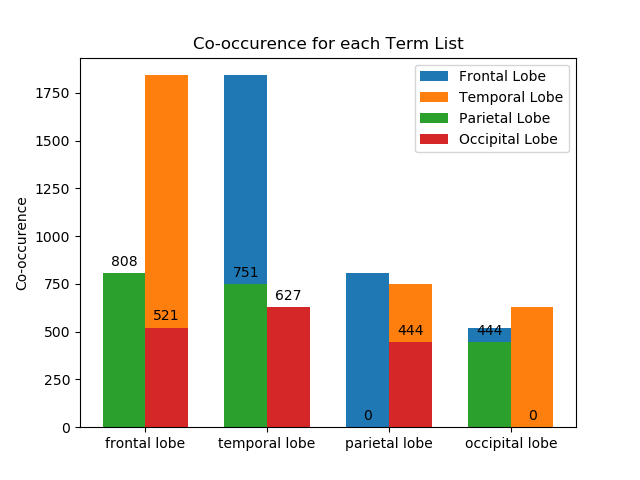
\includegraphics[width=0.9\textwidth]{counts}
  \caption{Matplotlib bar graph of the number of counts for word co-occurrence in the search term list.} 
  \label{fig:counts}
\end{figure}
%
We can also look at how many articles contain each of the specified search terms Figure~\ref{fig:document}. This figure shows the temperal lobe being the most studied part of the the brain.
%
\begin{figure}
  \centering
  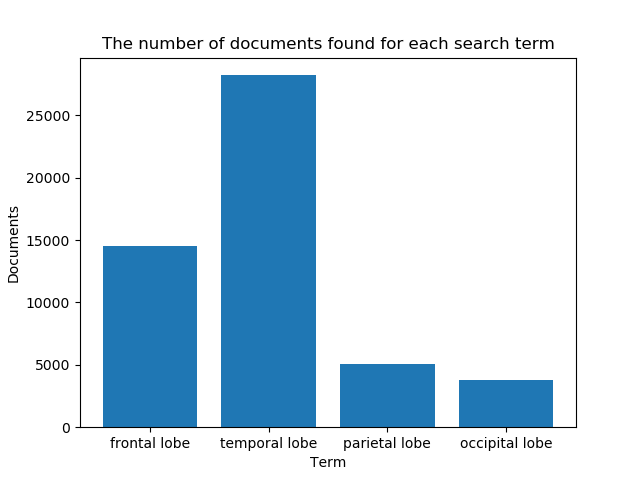
\includegraphics[width=0.9\textwidth]{document}
  \caption{Matplotlib bar graph of the number of documents found for each search term.}
  \label{fig:document}
\end{figure}
%
Another example of this packages function is it's ability to change NCBI databases, the above figures used the Pubmed database and Figure~\ref{fig:organism} uses the Nucleotide database. Nucleotide database hold genetic information about every studies species/organism on the planet. The example searched for five orgainisms and returned the number of articles that contained the search terms. Homo sapians have the highest number of articles written.
%
\begin{figure}
  \centering
  
\includegraphics[width=0.9\textwidth]{organism}
  \caption{Matplotlib graph of the number of articles that contain "Salmonella", "E.coli", "Sus scrofa", "Homo sapiens", and "Mus musculus".}
  \label{fig:organism}
\end{figure}
%
\section{Conclusions}

Lisc is a great tool to collect data on articles using several databases. It can plot the data in various formats to effectivly commmunicate the research completed.

\section{Reference}

Donoghue, T. (2018) LISC: A Python Package for Scientific Literature Collection and Analysis. Journal of Open Source Software, 4(41), 1674. DOI: 10.21105/joss.01674

\end{document}
